\section{Experimental Results}

\begin{enumerate}
        \item BBO-LP
        \item BUCB\footnote{The open source code only takes discret input, so we re-implemented the algorithm}
        \item qKG
        \item qEI
\end{enumerate}



\subsection{Benchmark Problems}

\begin{enumerate}
        \item Hart6
        \item Alpine1
        \item Branin
        \item Rosenbrock-2
        \item Rosenbrock-10
        \item Ackley-2
        \item Ackley-10
\end{enumerate}

\subsection{Operational Amplifier}

\textcolor{red}{TODO: qKG and qEI}

\begin{figure}[htbp]
\vskip 0.2in
\begin{center}
\centerline{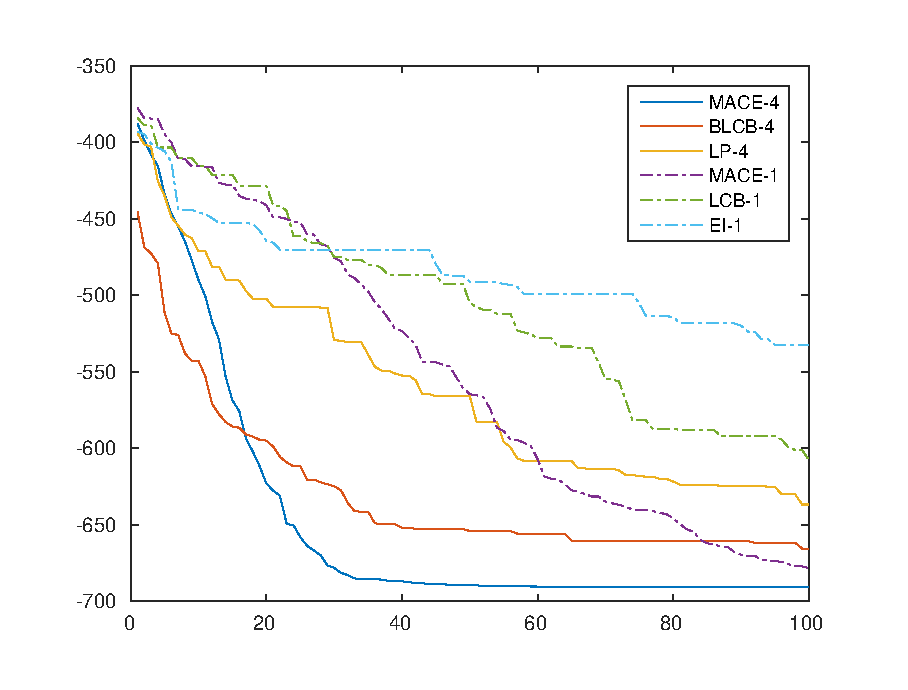
\includegraphics[width=\columnwidth]{./img/mean_DAC2014.eps}}
\caption{Optimization results of the operational amplifier}
\label{resDAC2014}
\end{center}
\vskip -0.2in
\end{figure}


\subsection{ClassE Power Amplifier}

\textcolor{red}{TODO: qKG and qEI}

\begin{figure}[htbp]
\vskip 0.2in
\begin{center}
\centerline{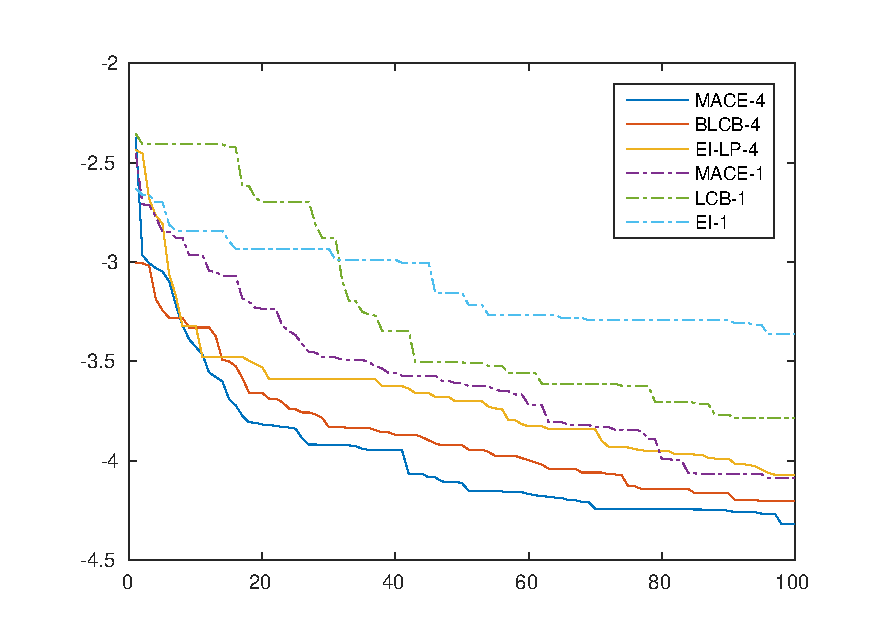
\includegraphics[width=\columnwidth]{./img/ClassE_mean.eps}}
\caption{Optimization results of the class-E power amplifier}
\label{resDAC2014}
\end{center}
\vskip -0.2in
\end{figure}

